%!TeX root=../main.tex
% -----------------------------------------------------------------------------
% sections/results.tex
% Purpose: Present results, plots, and key findings.
%
% Keep the narrative focused:
% - What was measured?
% - What are the key quantitative results?
% - What are the most important qualitative observations?
% -----------------------------------------------------------------------------

\section{Results}\label{sec:results}


\subsection{Main Results (Example Table)}\label{sec:main_results}

\begin{table}[H]
    \centering
    \caption{Example results table. Replace metrics and values with your own.}\label{tab:results}
    \begin{tabular}{lrr}
        \toprule
        Method & MSE $\downarrow$ & Runtime (s) $\downarrow$ \\
        \midrule
        Baseline & 0.123 & 12.4 \\
        Proposed & 0.101 & 13.1 \\
        \bottomrule
    \end{tabular}
\end{table}

\subsection{Trend Visualization (Example Plot)}\label{sec:trend_plot}

\pref{fig:learning_curves} is an example plot generated with \texttt{pgfplots}. Replace it with your actual figures.

\begin{figure}[H]
    \centering
    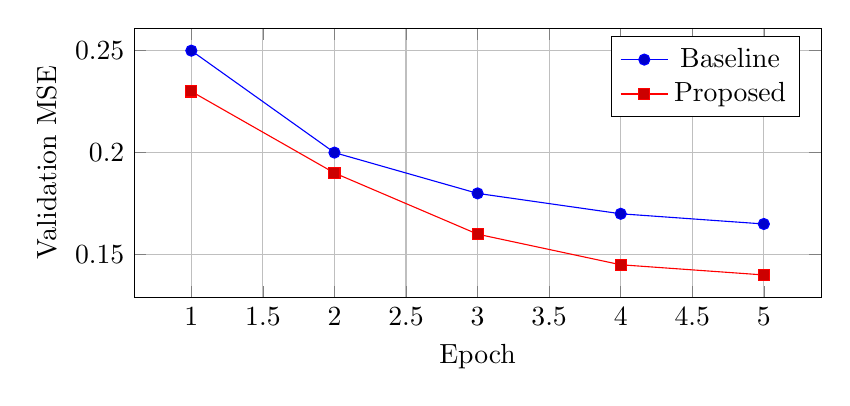
\begin{tikzpicture}
        \begin{axis}[
            width=0.85\linewidth,
            height=5cm,
            xlabel={Epoch},
            ylabel={Validation MSE},
            grid=both,
            legend pos=north east,
        ]
            \addplot+[mark=*] coordinates {
                (1,0.25) (2,0.20) (3,0.18) (4,0.17) (5,0.165)
            };
            \addlegendentry{Baseline}

            \addplot+[mark=square*] coordinates {
                (1,0.23) (2,0.19) (3,0.16) (4,0.145) (5,0.14)
            };
            \addlegendentry{Proposed}
        \end{axis}
    \end{tikzpicture}
    \caption{Example learning curves. Replace with your plot or a figure via \texttt{\string\includegraphics}.}\label{fig:learning_curves}
\end{figure}

\subsection{Key Takeaways}\label{sec:key_takeaways}

\begin{itemize}
    \item Finding 1.
    \item Finding 2.
    \item Finding 3.
\end{itemize}
